\chapter{Structural  Mechanics   model}
Static    structural   mechanics    problems   can    be   handled    using   the
\code{StructuralMechanicsModel}.  So far, \akantu\  provides 2D and 3D Bernoulli
beam elements \cite{frey2009}.  Just  as for the \code{SolidMechanicsModel}, the
model  is created  for  a given  \code{Mesh}.   The model  will  create its  own
\code{FEM}  object  to  compute  the interpolation,  gradient,  integration  and
assembly  operations.  The  \code{StructuralMechanicsModel} constructor  is used
like

\begin{cpp}
  StructuralMechanicsModel model(mesh, spatial_dimension);
\end{cpp}
where \code{mesh} is  a \code{Mesh} object defining the  structure for which the
equations  of statics  are to  be solved,  and \code{spatial\_dimension}  is the
dimensionality  of the  problem.  If  \code{spatial\_dimension} is  omitted, the
problem is assumed  to have the same dimensionality as the  one specified by the
mesh.

\note[\ 1]{Dynamic computations are not supported to date.}

\note[\ 2]{Structural meshes are created and loaded as described in
  Section~\ref{sect:common:mesh} with \code{MeshIOMSHStruct} instead  of \code{MeshIOMSH}.}

\vspace{1cm}
This model contains at least the following \code{Vectors}:
\begin{description}
\item[boundary]  contains a  boolean  value for  each  degree of  freedom
  specifying  whether  that degree  is  blocked  or  not. A  Dirichlet  boundary
  condition can be prescribed by setting the \textbf{boundary} value of a degree
  of freedom to  \code{true}.  A Neumann boundary condition  can  be applied
  by setting the corresponding  \textbf{boundary} value to  \code{false}.
  The \textbf{displacement} is computed for all degrees of freedom for which the \textbf{boundary} value is set to \code{false}. For the remaining degrees of freedom, the imposed values (zero by default after initialization) are kept.
  

  
\item[displacement\_rotation]  contains  the  generalized displacements (displacements and rotations)  of  all
  degrees of freedom. It can be  either a computed displacement for free degrees
  of freedom  or an imposed displacement  in case of blocked  ones ($\vec{u}$ in
  the following).
  
\item[force\_moment]  contains the  generalized external  forces (forces and moments) applied  to the
  nodes ($\vec{f_{\st{ext}}}$ in the following).
  
\item[residual] contains the difference between external and internal forces and
  moments. On the blocked degrees of freedom, \textbf{residual} contains the support
  reactions   ($\vec{r}$ in  the following).   It should  be mentioned  that at
  equilibrium, \textbf{residual} should be zero on the free degrees of freedom.
\end{description}

An example to help understand how  to use this model will be presented in the
next section.

\section{Model setup}
\label{sec:structMechMod:setup}

\subsection{Initialization}
The easiest way to initialize the structural mechanics model is:
%\begin{cpp}
%  model.initModel();
%  
%  StructuralMaterial mat1;
%  mat1.E=2.05e11;
%  mat1.I=0.00128;
%  mat1.A=0.01; // for example
%
%  model.addMaterial(mat1); ASK NICO ABOUT THIS CRAP
%
%  model.initVectors();
%  model.initImplicitSolver();
%\end{cpp}
%The method \code{initModel} computes the shape functions, \code{addMaterial} sets the material parameters to be used, \code{initVectors} initializes all the internal vectors mentioned before and \code{initImplicitSolver} creates the stiffness matrix.

\begin{cpp}
  model.initFull();
\end{cpp}
The method \code{initFull} computes the shape functions, initializes the internal vectors mentioned above and allocates the memory for the stiffness matrix.

Material  properties are  defined using  the \code{StructuralMaterial}
structure described in Table~\ref{tab:structMechMod:strucMaterial}. Such a definition could for instance look like
\begin{cpp}
  StructuralMaterial mat;
  mat.E=3e10;
  mat.I=0.0025;
  mat.A=0.01;
\end{cpp}

\begin{table}[htb] \centering
  \begin{tabular}{c|c} field  & description \\\hline\hline
    \code{E} & Young's  modulus  \\\hline
    \code{A}  & Cross  section  area  \\\hline
    \code{I} & Second cross sectional  moment of inertia (for 2D elements)
    \\\hline \code{Iy} & \code{I}  around beam $y$--axis (for 3D elements)
    \\\hline \code{Iz} & \code{I}  around beam $z$--axis (for 3D elements)
    \\\hline \code{GJ}  & Polar  moment of inertia  of beam  cross section (for 3D elements)
  \end{tabular}
  \caption{Material properties  for structural elements  as defined by
the structure \code{StructuralMaterial}.}
  \label{tab:structMechMod:strucMaterial}
\end{table}
Materials can be added to the model's \code{element\_material} vector using
\begin{cpp}
  model.addMaterial(material);
\end{cpp}

They are used just like for the \code{SolidMechanicsModel}
see Section~\ref{sect:smm:CL}.
\subsection{Setting boundary conditions}\label{sect:structMechMod:boundary}

Both Dirichlet  and Neumann  type boundary conditions  are applied to  nodes the
same     exact    way     as     for    \code{SolidMechanicsModel},     see
Section~\ref{sect:smm:boundary}.   The  method  \code{computeForcesFromFunction}
can still be used to apply Neumann boundary conditions.

\section{Static analysis\label{sect:structMechMod:static}}

The  \code{StructuralMechanicsModel}  class   can  perform  static  analyses  of
structures.  In  this case,  the  equation  to solve  is  the  same  as for  the
\code{SolidMechanicsModel} used for static analyses
\begin{equation}\label{eqn:structMechMod:static}
  \mat{K} \vec{u} = \vec{f_{\st{ext}}}~,
\end{equation}
where  $\mat{K}$ is  the  global stiffness  matrix,  $\vec{u}$ the  generalized displacement 
vector  and  $\vec{f_{\st{ext}}}$ the  vector of generalized external  forces   applied to  the
system.


To     solve    such     a    problem,     the    static     solver     of    the
\code{StructuralMechanicsModel}\index{StructuralMechanicsModel}  object is used.   First a
model has to be  created and initialized.  To create the model,  a mesh is required.
Once an instance of a \code{StructuralMechanicsModel} is obtained, the easiest way to
initialize it is  to use the \code{initFull}\index{StructuralMechanicsModel!initFull}
function.

\begin{cpp}
  StructuralMechanicsModel model(mesh);
  model.initFull();
\end{cpp}


\begin{itemize}
\item \code{model.initFull}  initializes all internal vectors to zero.
\end{itemize}


Once the model is created and  initialized, the boundary conditions can be set as
explained   in  Section   \ref{sect:structMechMod:boundary}.   Boundary   conditions  will
prescribe   the   external   forces or moments    for   the   free   degrees   of   freedom
$\vec{f_{\st{ext}}}$ and displacements or rotations for the others.  To completely define the
system  represented  by equation  (\ref{eqn:structMechMod:static}),  the global  stiffness
matrix            $\mat{K}$             must            be            assembled.
\index{StructuralMechanicsModel!assembleStiffnessMatrix}

\begin{cpp}
  model.assembleStiffnessMatrix();
\end{cpp}

The computation of the static equilibrium is performed using the same
Newton-Raphson algorithm as described in
Section~\ref{sect:smm:static}.

\note{To date,
\code{StructuralMechanicsModel} handles only constitutively and
geometrically linear problems, the algorithm is therefore guaranteed
to converge in one iteration.}

\begin{cpp}
  model.updateResidual();
  model.solve();
\end{cpp}
\index{StructuralMechanicsModel!updateResidual}
\index{StructuralMechanicsModel!solve}

\begin{itemize}
\item \code{model.updateResidual} assembles the  internal forces and removes them
  from the external forces.
\item        \code{model.solve}         solves        the        equations
  (\ref{eqn:smm:static-newton-raphson}).   The \textbf{increment} vector  of the
  model   will   contain  the   new   increment   of   displacements,  and   the
  \textbf{displacement} vector is also updated to the new displacements.
\end{itemize}

At   the  end   of  the   analysis, the   final  solution   is  stored   in  the
\textbf{displacement}  vector.  A  full example  of  how to  solve a  structural
mechanics       problem        is       presented       in        the       code
\code{\examplesdir/WHERE-DO-EXAMPLES-GO?}\todo{set the right example file}.  This  example is composed  of a 2D
beam, clamped at  the left end and  supported by two rollers as  shown in Figure
\ref{fig:structMechMod:exem1_1}.  The problem  is  defined by  the applied  load
$q=\unit{6}{\kilo\newton\per\metre}$,          moment         $\bar{M}         =
\unit{3.6}{\kilo\newton\metre}$,      moments     of     inertia      $I_1     =
\unit{250\,000}{\power{\centi\metre}{4}}$           and          $I_2          =
\unit{128\,000}{\power{\centi\metre}{4}}$ and  lengths $L_1 = \unit{10}{\metre}$
and $L_2 = \unit{8}{\metre}$.  The resulting rotations at node two and three are
$ \varphi_2 = 0.001\,167\ \mbox{and}\ \varphi_3 = -0.000\,771.$


 \begin{figure}[htb]
   \centering
   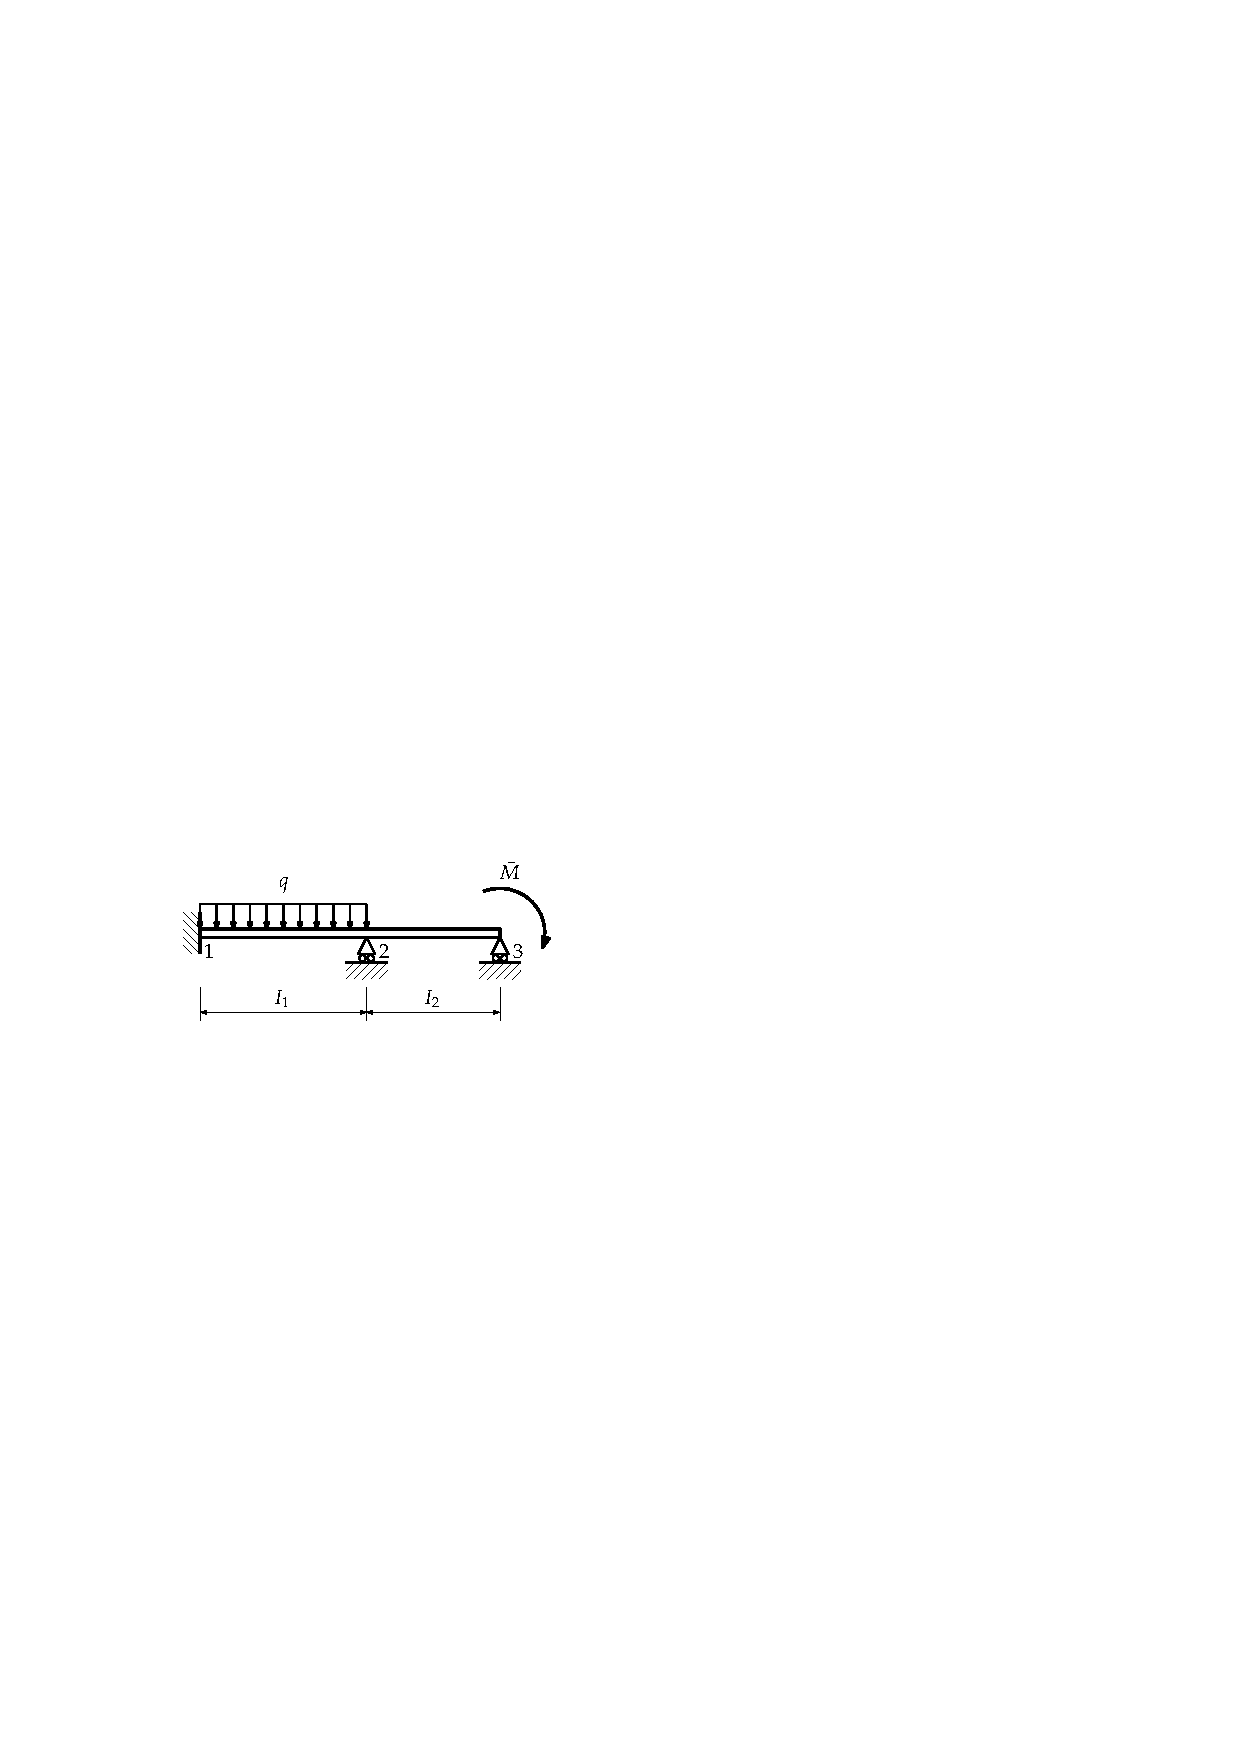
\includegraphics[scale=1.1]{figures/beam_example}
   \caption{2D beam example}
   \label{fig:structMechMod:exem1_1}
 \end{figure}





%%% Local Variables:
%%% mode: latex
%%% TeX-master: "manual"
%%% End:


